\documentclass{article}
\author{Alejandro Zubiri}
\date{Fri Nov 08 2024}
\title{Inferencia}

\usepackage{amsmath, amsfonts, amsthm, graphicx}

\graphicspath{{../images/}}

\begin{document}
\maketitle
\tableofcontents
\pagebreak
La inferencia es el estudio de lo poco que conocemos para sacar conclusiones de lo mucho que desconocemos.
\section{Estimación}
Sirve para hacer prediciones sobre parámetros de la población.\\
El estimador de un parámetro $\theta $ es una función de los valores de la muestra para estimar $\theta $. Un estimador
se denota por $\hat{\theta }$
\begin{equation}
    \begin{split}
        \hat{\theta }=g(x_{1},\dots,x_{n})
    \end{split}
\end{equation}
Cuanto más aproximado es un estimador al próximo parámetro, decimos que es \textbf{insesgado}. Si un estimador lo es
se verifica que
\begin{equation}
    \begin{split}
        E(\hat{\theta })=\theta 
    \end{split}
\end{equation}
Donde $E(\hat{\theta })$ es la esperanza (media) del estimador.\\
Una de las propiedades es que:
\begin{equation}
    \begin{split}
        E(\hat{\theta })= \theta +b(\theta )
    \end{split}
\end{equation}
Donde $b(\theta )$ es el sesgo ("error").\\
También tenemos la \textbf{varianza mínima} o \textbf{precisión}, que es la proximidad entre muestras repetidas.
Calculamos el error de muestreo como:
\begin{equation}
    \begin{split}
        e(\hat{\mu })= \frac{\sigma }{\sqrt{n}}
    \end{split}
\end{equation}
Y finalmente la \textbf{eficiencia}, que es un estimador insesgado de varianza mínima:
\begin{equation}
    \begin{split}
        efic(\hat{\theta })= \frac{1}{var(\hat{\theta })}
    \end{split}
\end{equation}
Un ejemplo de estimador eficiente y lineal es el \textbf{ELIO}.\\
El criterior para un estimador es el \textbf{error cuadrático medio} (ECM):
\begin{equation}
    \begin{split}
        ECM(\hat{\theta })= E((\hat{\theta }-\theta )^{2})= var(\hat{\theta })+ b^{2}(\hat{\theta })
    \end{split}
\end{equation}
\begin{proof}[Distribución muestral]
    Distribución de probabilidad de un estadístico
\end{proof}
\subsection{Varianza conocida}
Sea una variable aleatoria:
\begin{equation}
    \begin{split}
        E(\bar{X}) = \frac{E(X_{1})+E(X_{2})+\dots+E(X_{n})}{n}= \frac{\mu +\mu +\dots+\mu }{n}
        = \frac{n \mu }{n} = \mu 
    \end{split}
\end{equation}
\begin{equation}
    \begin{split}
        var(\bar{X})= \frac{var(X_{1}+X_{2}+\dots +X_{n})}{n^{2}}= \frac{\sigma^{2}+\dots+\sigma^{2}}{n^{2}}
        = \frac{n \sigma^{2}}{n^{2}}= \frac{\sigma^{2}}{n}
    \end{split}
\end{equation}
\begin{proof}[Teorema central del límite]
    Sean $x_{1},x_{2},\dots,x_{n}$ variables independientes identicamente distribuidas, con media
    $\mu _{i}$ y con desviación típica $\sigma _{i}$:
    \begin{equation}
        \begin{split}
            \frac{\sum x_{i}-\sum \mu _{i}}{\sqrt{\sum \sigma^{2}}} \to N(0,1)
        \end{split}
    \end{equation}
    Si $n$ es grande $(n>30)$, es asintóticamente normal:
    \begin{equation}
        \begin{split}
            \bar{X} \to N(\mu , \frac{\sigma }{\sqrt{n}})
        \end{split}
    \end{equation}
    Si la población ya es normal, se cumple siempre
\end{proof}
\subsection{Varianza desconocida}
Si la varianza es desconocida, usamos la varianza muestral $\hat{S}^{2}$:
\begin{equation}
    \begin{split}
        \frac{\bar{X}-\mu }{\hat{S} / \sqrt{n}} \to t_{n-1}
    \end{split}
\end{equation}
Donde $t$ es la $t$ de Student.
\subsection{Distribución muestral de proporción}
Si $p$ es la proporción de individuos que cumplen una determinada característica:
\begin{equation}
    \begin{split}
        \hat{p}= \frac{\sum x_{i}}{n} = \bar{X}
    \end{split}
\end{equation}
Donde $x_{i}$ es aleatoria y toma $0$ o $1$.\\
Si $n>30$ y $np(1-p)>5$, aplicamos el teorema central del límite:
\begin{equation}
    \begin{split}
        \frac{p-\hat{p}}{\sqrt{\hat{p}(1-\hat{p}) / n}} \approx N(0,1)
    \end{split}
\end{equation}
\subsection{Distribución muestral de la varianza}
\begin{equation}
    \begin{split}
        \hat{S}^{2} = \frac{\sum x_{i} -\bar{x}}{n-1}
    \end{split}
\end{equation}
Es el estimador insesgado de varianza poblacional. Cuando la muestra viene de una distribución
normal:
\begin{equation}\tag*{Lema de Fisher-Cochran}
    \begin{split}
        \frac{S^{2}}{\sigma^{2}} \approx \frac{\chi^{2}_{n-1}}{n-1}
    \end{split}
\end{equation}
\subsection{Intervalos de confianza}
Queremos la media $\mu $ de una población, \textbf{pero no podemos}. Como alternativa,
calculamos la media con incertidumbre (probabilidad):\\
Para el parámetro $\theta $ con nivel de confianza $1-\alpha $, es el intervalo
$\theta_{1}(X), \theta _{2} (X)$ tal que:
\begin{equation}
    \begin{split}
        P(\theta _{1}(X) \leq \theta \leq \theta _{2}(x)) = 1-\alpha 
    \end{split}
\end{equation}
Donde $\alpha $ es el nivel de significación.
\subsubsection{Cálculo de los intervalos - media con $\sigma $ conocida}
Necesitamos un pivote:
\begin{itemize}
    \item Que incluya lo que queremos calcular: $\mu $
    \item Que incluya lo que conocemos: $\bar{x}$
    \item Una distribución conocida
\end{itemize}
\begin{equation}
    \begin{split}
        \bar{x}\to N(\mu , \frac{\sigma }{\sqrt{n}})
    \end{split}
\end{equation}
\subsubsection{Cálculo de intervalos - media con $\sigma $ desconocida}
Si $n$ es grande:
\begin{equation}
    \begin{split}
        \bar{x} \pm Z_{1-\frac{\alpha }{2}} \frac{S_{x}}{\sqrt{n}}
    \end{split}
\end{equation}
Si $n$ es pequeña pero dada por una distribución normal:
\begin{equation}
    \begin{split}
        IC(\mu _{x}) = (\bar{x}\pm t_{n-1,1-\frac{\alpha }{2}})\cdot \frac{S_{x}}{\sqrt{n}}
    \end{split}
\end{equation}
Para definir $Z_{1-\frac{\alpha }{2}}$:
\begin{equation}
    \begin{split}
        p(Z> Z_{1-\frac{\alpha }{2}}) = \frac{\alpha}{2}
    \end{split}
\end{equation}
\begin{equation}
    \begin{split}
        p(Z < Z_{1-\frac{\alpha}{2}})= \frac{\alpha}{2}
    \end{split}
\end{equation}
\begin{equation}
    \begin{split}
        p(-Z_{1-\frac{\alpha}{2}} \leq \frac{\bar{X}-\mu _{x}}{\sigma _{x} / \sqrt{n}}\leq Z_{1-\frac{\alpha}{2}})= 1-\alpha 
    \end{split}
\end{equation}
\begin{equation}
    \begin{split}
        IC_{1-\alpha }(\mu _{x})= (\bar{x}\pm Z_{1-\alpha } \frac{\sigma _{x}}{\sqrt{n}})
    \end{split}
\end{equation}
\subsection{Para una proporción}
Nuestra media muestral será nuestra \textbf{media muestral}: $\bar{x}=\hat{p}$. Y
\begin{equation}
    \begin{split}
        \hat{\sigma }^{2}= p(1-p)
    \end{split}
\end{equation}
Entonces, en caso de contar con una muestra grande,
\begin{equation}
    \begin{split}
        IC(p_{x}) = (\hat{p}_{x} \pm Z_{1-\alpha / 2} \sqrt{\frac{\hat{p}(1-\hat{p})}{n}})
    \end{split}
\end{equation}
\section{Varianza en poblaciones normales}
Contando con el teorema de Fisher-Cochran:
\begin{equation}
    \begin{split}
        \frac{(n-1)S^{2}}{\sigma^{2}} \approx \chi^{2}_{n-1}
    \end{split}
\end{equation}
Llamamos a $\chi^{2}_{(n-1, 1-\alpha /2)}$ y $\chi^{2}_{(n-1, \alpha /2)}$ los valores que
dejan una probabilidad de $1-\alpha $:
\begin{equation}
    \begin{split}
        p(\frac{(n-1)S^{2}}{\chi^{2}_{(n-1, 1-\alpha /2)}} \geq \sigma^{2} \geq
        \frac{(n-1)S^{2}}{\chi^{2}_{(n-1, \alpha /2)}})=1-\alpha 
    \end{split}
\end{equation}
\section{Contraste de hipótesis}
Tenemos dos alternativas:
\begin{itemize}
    \item $H_{0}$: nula o neutra. Se contraste, y la mantenemos a menos que se demuestre lo
    contrario, sino se acepta.
    \item $H_{1}$: alternativa. Se acepta si se deniega la neutra.
\end{itemize}
\pagebreak
\subsection{Método}
La hipótesis nula es verdadera hasta que se demuestra lo contrario.\\
Una discrepancia grande tiene poca probabilidad de ocurrir si la hipótesis es nula:
\begin{center}
    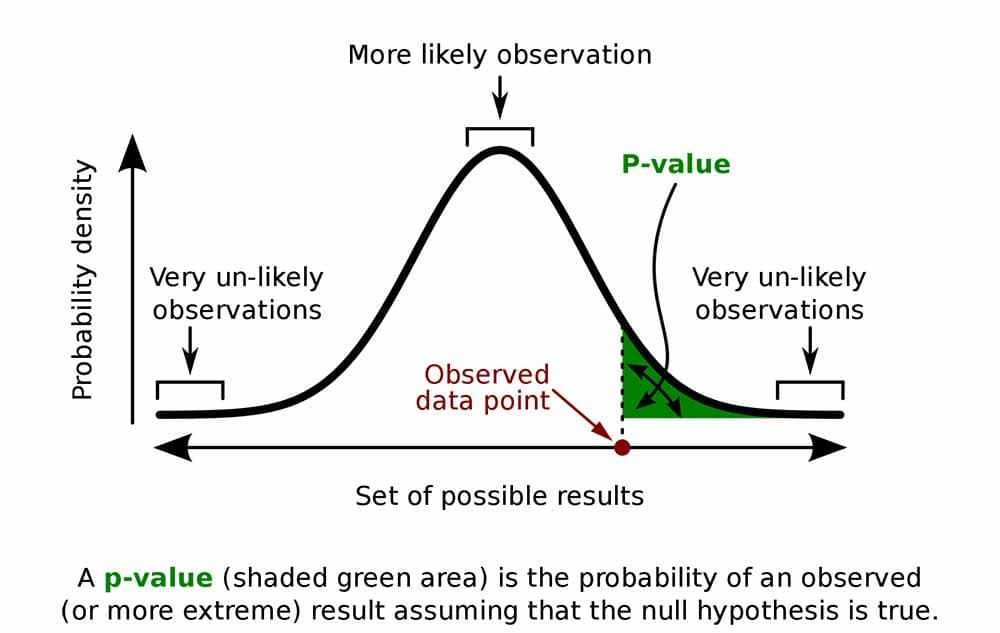
\includegraphics[scale=0.25]{p-value.jpg}
\end{center}
Hay dos tipos de errores:
\begin{itemize}
    \item Rechazar hipótesis verdadera: tipo I $(\alpha )$
    \item Aceptar hipótesis falsa: Tipo II
\end{itemize}
Y definimos $\alpha $ como:
\begin{equation}
    \begin{split}
        \alpha = p(\frac{\text{Rechazar }H_{0}}{H_{0}\text{ cierta}})
    \end{split}
\end{equation}
\subsection{Valor $p$}
Es la región de rechazo, el \textbf{nivel crítico} ($p$-valor).
\begin{proof}[$p$-valor]
    Probablidad de obtener discrepancia mayor o igual que la observada si $H_{0}$ es cierta.\\
    $p<0.05$: poca evidencia, la rechazamos.
\end{proof}
\subsection{Cálculo de contrastes}
\subsubsection{Media con $\sigma $ conocida}
Contrastamos la hipótesis, sabiendo que la media de la distribución es $\mu_{0}$
\textbf{Primer caso}:
\begin{equation}
    \begin{split}
        H_{0}:& \mu = \mu_{0}\\ H_{1}:& \mu \neq \mu_{0}
    \end{split}
\end{equation}
Sabemos que:
\begin{equation}
    \begin{split}
        \frac{\bar{x}-\mu }{\sigma / \sqrt{n}} \approx N(0,1)
    \end{split}
\end{equation}
Por tanto, rechazamos $H_{0}$ si:
\begin{equation}
    \begin{split}
        Z &> Z_{1-\alpha / 2}\\ Z &< -Z_{1- \alpha /2}
    \end{split}
\end{equation}
\textbf{Segundo caso}:
\begin{equation}
    \begin{split}
        H_{0}&: \mu \leq \mu_{0}\\ H_{1}&: \mu > \mu_{0}
    \end{split}
\end{equation}
En este caso, rechazaremos la hipótesis si:
\begin{equation}
    \begin{split}
        \frac{\bar{x}-\mu_{0}}{\sigma / \sqrt{n}}> Z_{1-\alpha }
    \end{split}
\end{equation}
\textbf{Tercer caso}:
\begin{equation}
    \begin{split}
        H_{0}&: \mu \geq \mu_{0}\\ H_{1}&: \mu < \mu_{0}
    \end{split}
\end{equation}
La rechazaremos si:
\begin{equation}
    \begin{split}
        \frac{\bar{x}-\mu_{0}}{\sigma / \sqrt{n}}< -Z_{1-\alpha }
    \end{split}
\end{equation}
\subsubsection{Media con $\sigma $ desconocida}
Partiendo de una población que debe ser normal:
\begin{equation}
    \begin{split}
        \frac{\bar{x}-\mu }{\hat{S} / \sqrt{n}}\approx t_{n-1}
    \end{split}
\end{equation}
Rechazamos la hipótesis nula $H_{0}$ si:
\begin{equation}
    \begin{split}
        \frac{\bar{x}-\mu }{\hat{S} / \sqrt{n}}&>t_{n-1,1-\alpha /2}\\
        \frac{\bar{x}-\mu }{\hat{S} / \sqrt{n}}&<t_{n-1,\alpha /2}
    \end{split}
\end{equation}
\subsubsection{Contraste para una proporción}
Ya sabemos que para una proporción:
\begin{equation}
    \begin{split}
        \frac{\hat{p}-p_{0}}{\sqrt{p_{0}(1-p_{0}) / \sqrt{n}}}\approx N(0,1)
    \end{split}
\end{equation}
si la muestra es suficientemente grande. En estos casos, rechazaremos la hipótesis nula si:
\begin{equation}
    \begin{split}
        \frac{\hat{p}-p_{0}}{\sqrt{p_{0}(1-p_{0}) / \sqrt{n}}} &> Z_{1-\alpha /2}\\
        \frac{\hat{p}-p_{0}}{\sqrt{p_{0}(1-p_{0}) / \sqrt{n}}} &< -Z_{1-\alpha /2}
    \end{split}
\end{equation}
\subsubsection{Contraste para la varianza $\sigma^{2}$}
Ya sabemos que para la varianza:
\begin{equation}
    \begin{split}
        \frac{(n-1)S^{2}}{\sigma_{0}^{2}} \approx \chi^{2}_{n-1}
    \end{split}
\end{equation}
En caso de partir de una población normal. En este caso, rechazamos la hipótesis si:
\begin{equation}
    \begin{split}
        \frac{(n-1)S^{2}}{\sigma_{0}^{2}} &> \chi^{2}_{n-1, 1-\alpha /2}\\
        \frac{(n-1)S^{2}}{\sigma_{0}^{2}} &< \chi^{2}_{n-1, \alpha /2}
    \end{split}
\end{equation}
\subsubsection{Contraste para el tamaño muestral}
El tamaño muestral es el número de elementos del universo que se seleccionan para cada muestra.\\
Para aproximar la media, tenemos que:
\begin{equation}
    \begin{split}
        \frac{rango}{4} \approx \sigma 
    \end{split}
\end{equation}
Aunque la $\sigma $ real siempre será menor. Para el caso de proporciones, siempre se asume el caso más
desfavorable: $p=q=0.5$.\\
Se considera \textbf{universo grande} cuando:
\begin{equation}
    \begin{split}
        N &\geq 100n\\
        N &\geq 20n
    \end{split}
\end{equation}
Para calcular el tamaño de la muestra, este será:
\begin{equation}
    \begin{split}
        \boxed{n = \frac{Z^{2}_{1-\frac{\alpha}{2} }\sigma^{2}}{e^{2}}}
    \end{split}
\end{equation}
Esto se aplica también para una proporción, donde
\begin{equation}
    \begin{split}
        \sigma^{2} = \hat{p}(1-\hat{p})
    \end{split}
\end{equation}
Para el caso de \textbf{universo pequeño}, debemos aplicar la corrección:
\begin{equation}
    \begin{split}
        \frac{N-n}{N-1}
    \end{split}
\end{equation}
Donde $N$ es el tamaño de la población y $n$ el de la muestra. Con esta corrección, el tamaño
sería
\begin{equation}
    \begin{split}
        \boxed{n = \frac{N Z^{2}_{1-\alpha /2} \sigma^{2}}{(N-1)e^{2}+Z^{2}_{1-\alpha /2}\sigma^{2}}}
    \end{split}
\end{equation}
\section{Resumen de intervalos}
\begin{itemize}
	\item Media con varianza: $Z_{1-\alpha / 2}$
	\item Media sin varianza:
		\begin{itemize}
			\item Con DNORM: $t_{n-1}$
			\item Con $n$ grande: $Z_{1-\alpha / 2}$  
		\end{itemize}
	\item Proporción con $n$ grande: $Z_{1-\alpha / 2}$
	\item Varianza con DNORM: $ \frac{(n-1)S^{2}}{\chi^{2}_{n-1, 1-\alpha / 2}}$
\end{itemize}
\section{Resumen de contrastes}
\begin{itemize}
	\item Media con varianza: $Z_{1-\alpha / 2}$
	\item Media sin varianza con DNORM: $t_{n-1, 1-\alpha / 2}$
	\item Proporción con $n$ grande: $Z_{1-\alpha / 2}$
	\item Varianza con DNORM: $\chi^{2}_{n-1,1-\frac{\alpha}{2}}$ 
\end{itemize}
\section{Afijación}
Es la distribución del número de individuos por muestra:
\subsubsection{Simple}
Dividimos el total entre el número de estratos:
\begin{equation}
    \begin{split}
        n_{i} = \frac{n}{L}
    \end{split}
\end{equation}
donde $L$ es el número de estratos.
\subsubsection{Proporcional}
Lo ponderamos con lo proporcional que sea cada estrato:
\begin{equation}
    \begin{split}
        n_{i} = n \frac{N_{i}}{N}
    \end{split}
\end{equation}
Donde $N_{i}$ es la población del estrato $i$.
\subsubsection{Óptima o de Neyman}
Ponderamos cada estrato por la varianza:
\begin{equation}
    \begin{split}
        n_{i} = n \frac{N_{i}\sigma _{i}}{\sum N_{i}\sigma _{i}}
    \end{split}
\end{equation}
\section{Error de muestreo para la estimación}
\begin{itemize}
    \item Universo grande:
    \begin{equation}
        \begin{split}
            e_{x} = \frac{\sigma }{\sqrt{n}}
        \end{split}
    \end{equation}
    \item Universo pequeño:
    \begin{equation}
        \begin{split}
            e_{x} = \frac{\sigma }{\sqrt{n}} \sqrt{\frac{N-n}{N-1}}
        \end{split}
    \end{equation}
\end{itemize}
Esto funcionará igual para la proporción, donde $\sigma^{2} = p(1-p)$.
\end{document}
